%!TEX program = Xelatex
\documentclass{article}
%\usepackage{ctex}
\usepackage{amsmath,amscd,amsbsy,amssymb,latexsym,url,bm,amsthm}
\usepackage{epsfig,graphicx,subfigure}
\usepackage{enumitem,balance,mathtools}
\usepackage{wrapfig}
\usepackage{mathrsfs, euscript}
\usepackage[usenames]{xcolor}
\usepackage{hyperref}
\usepackage{caption}
\usepackage{setspace}
%\usepackage{subcaption}
\usepackage{float}
\usepackage{listings}
%\usepackage{enumerate}
%\usepackage{algorithm}
%\usepackage{algorithmic}
%\usepackage[vlined,ruled,commentsnumbered,linesnumbered]{algorithm2e}
\usepackage[ruled,lined,boxed,linesnumbered]{algorithm2e}

\newtheorem{theorem}{Theorem}[section]
\newtheorem{lemma}[theorem]{Lemma}
\newtheorem{proposition}[theorem]{Proposition}
\newtheorem{corollary}[theorem]{Corollary}
\newtheorem{exercise}{Exercise}[section]
\newtheorem*{solution}{Solution}

\renewcommand{\thefootnote}{\fnsymbol{footnote}}
\renewenvironment{solution}[1][Solution]{~\\ \textbf{#1.}}{~\\}

\newcommand{\postscript}[2]
    {\setlength{\epsfxsize}{#2\hsize}
    \centerline{\epsfbox{#1}}}

\renewcommand{\baselinestretch}{1.0}
\SetKwFor{Function}{function}{:}{end}
\setlength{\oddsidemargin}{-0.365in}
\setlength{\evensidemargin}{-0.365in}
\setlength{\topmargin}{-0.3in}
\setlength{\headheight}{0in}
\setlength{\headsep}{0in}
\setlength{\textheight}{10.1in}
\setlength{\textwidth}{7in}

\title{CS222 Homework 3}
\author{Algorithm Analysis \& Deadline: 2020-10-09 Firday 24:00}
\date{Exercises for Algorithm Design and Analysis by Li Jiang, 2020 Autumn Semester}

\begin{document}

\maketitle

\begin{enumerate}

\item Given an integer array, please use the divide and conquer algorithm to find the reverse pair in the sequence.
~\\
\begin{solution}
    We use the divide and conquer algorithm to find the \textbf{number} of reverse pairs. (To find all of the reverse pairs needs $O(n^2)$, so divide and conquer algorithm has no advantages in this task. But to find the number of reverse pairs only needs $O(n\log n)$).\\
    \begin{minipage}[H]{0.8\textwidth}
        \begin{algorithm}[H]
            \caption{merge-sort-count-reverse-pair}\label{mergesort}
            \KwIn{A sequence $L=(l_1,l_2,l_3,\cdots,l_n)$}
            \KwOut{The number of reverse pairs in $L$, and the sorted sequence $L'$}
            \BlankLine
            \Function{Sort-And-Count(L)}{
                \BlankLine
                \If{$|L|=1$}{
                    \Return{(0, L)}
                }
                Divide $L$ into two halves $L1=(l_1,l_2,\cdots,l_{\lfloor\frac{n}{2}\rfloor})$, $L2=(l_{\lfloor\frac{n}{2}\rfloor+1},\cdots,l_n)$\\
                $(c_1,L1')\leftarrow$ Sort-And-Count($L1$)\\
                $(c_2,L2')\leftarrow$ Sort-And-Count($L2$)\\
                $(c, L')\leftarrow$ Merge-And-Count($L1'$,$L2'$)\\
                \Return{$(c+c_1+c_2, L')$}\\
            }
            \BlankLine
            \BlankLine
            \BlankLine
            \Function{Merge-And-Count(L1,L2)}{
                \BlankLine
                $count \leftarrow 0$\\
                $L \leftarrow$ an empty sequence\\
                \While{$L1$ \rm{is not empty} \rm{\textbf{OR}} $L2$ is not empty}{
                    \If{$L1$ is empty}{
                        Move the first elements of $L2$ to the tail of $L$
                    }
                    \ElseIf{$L2$ is empty}{
                        Move the first elements of $L1$ to the tail of $L$
                    }
                    \Else{
                        \If{(the first element of $L1$) $\prec$ (the first element of $L2$)}{
                            Move the first elements of $L1$ to the tail of $L$
                        }
                        \Else{
                            Move the first elements of $L2$ to the tail of $L$\\
                            $count\leftarrow count + $ (the number of elements in $L1$)
                        }
                    }
                }
                \Return{$(count, L)$}
            }

        \end{algorithm}
    \end{minipage}\\
    $T(2n)=2T(n)+2n\Rightarrow T(n)=\Theta(n\log n)$
\end{solution}
~\\
\newpage
\item Given any positive integers $K$ and $M$, find the $K$-th largest element and the $M$-th smallest element in the unsorted array. Please note that you need to find the $K$-th largest element, and the $M$-th smallest element after the array is sorted, not different elements.

~\\
\begin{solution}
    Like quick-sort, we choose a number $x$ from the array randomly (or just choose the first number in the array), and divide the array to two part: the left one contains the number smaller than $x$, the right one contains the number larger than $x$. \\
    \begin{minipage}[H]{0.8\textwidth}
        \begin{algorithm}[H]
            \caption{Find-M-th-smallest-element}
            \label{quicksort-divide}
            \KwIn{An unsorted array $A=(a_1,a_2,a_3,\cdots,a_n)$, a positive interger $M$}
            \KwOut{The M-th smallest element $x$}
            \BlankLine
            \Function{Find-M-th-smallest(A, M)}{
                \BlankLine
                $L1\leftarrow$ empty array\\
                $L2\leftarrow$ empty array\\
                \For{$element$ \rm{\textbf{in}} $A$}{
                    \If{$element \prec a_1$}{
                        Add $element$ to $L1$
                    }
                    \Else{
                        Add $element$ to $L2$
                    }
                }
                \If{(the number of elements in $L1$) $=M-1$}{
                    \Return{$a_1$}
                }
                \If{(the number of elements in $L1$) $<M-1$}{
                    \Return{Find-M-th-smallest($L2$, $M-1-$(the number of elements in $L1$))}
                }
                \If{(the number of elements in $L1$) $>M-1$}{
                    \Return{Find-M-th-smallest($L1$, $M$)}
                }
            }
        \end{algorithm}
    \end{minipage}\\
    To find the $K$-th largest one, we call Find-M-th-smallest($A$, $length(A)+1-K$).\\
    In the worst situation, it is $O(n^2)$. However in average situations, it is efficient (it is linear).\\
    Let $T(n):=\sup_k \mathbb{E}T(n,k)$, then we have 
    \begin{spacing}{2.0}
    \begin{equation}
        \begin{array}{ll}T(n)&=n+\dfrac{1}{n}\sum_{i=1}^{n}{\left(\mathbb{I}\{i<k\}\cdot \mathbb{E}T(n-i,k-i)+\mathbb{I}\{i>k\}\cdot \mathbb{E}T(i-1,k)\right)}\\ &\leq n+\dfrac{1}{n}\sum_{i=1}^{n}{(\mathbb{I}\{i<k\}\cdot T(n-i)+\mathbb{I}\{i>k\}\cdot T(i-1))}\\ &\leq n+\dfrac{1}{n}\sum_{i=1}^nT(\max\{n-i,i-1\})\\ & = n+\dfrac{2}{n}\sum_{i=\lfloor\frac{n}{2}\rfloor}^{n-1} T(i) \\\end{array}
    \end{equation}
    \end{spacing}
    $T(n)\leq cn \Rightarrow T(n+1)\leq n+1+\dfrac{2}{n+1}\times\dfrac{3c}{8}n^2\leq \left(1+\dfrac{3c}{4}\right)(n+1)\leq c(n+1)$, for $c>4$.\\
    Therefore $T(n) = O(n)$.
\end{solution}
~\\
\newpage
\item Given an array of linked lists, and the lists have been sorted in descending order. Please merge all linked lists into an ascending list and return the merged list.

~\\
\begin{minipage}[H]{0.8\textwidth}
    \begin{algorithm}[H]
        \caption{Merge-lists}
        \label{merge-list}
        \KwIn{An array of linked lists $L=(l_1,l_2,\cdots,l_n)$}
        \KwOut{Merged list $L'$}
        \BlankLine
        \Function{Merge-list(L)}{
            \BlankLine
            \If{$|L|=1$}{
                \Return{Ascending($l_1$)}
            }
        
            Choose two shortest links $l_i, l_j$ from $L$.\\
            $l'\leftarrow$ Merge-two(Ascending($l_i$), Ascending($l_j$))\\
            \Return{Merge-list($L-\{l_i\}-\{l_j\}+\{l'\}$)}\\
        }
        \BlankLine
        \Function{Ascending(l)}{
            \BlankLine
            \If{$|l|=1$ \textbf{OR} $l_1<l_2$}{
                \Return{l}
            }
            \Else{
                Reverse l\\
                \Return{l}
            }
        }
        \BlankLine
        \Function{Merge-two(l1, l2)}{
            \BlankLine
            $L\leftarrow $ an empty link.\\
            \While{$l1$ is not empty \textbf{OR} $l2$ is not empty}{
                \If{$l1$ is empty}{
                    Move the first element of $l2$ to the tail of $L$
                }
                \ElseIf{$l2$ is empty}{
                    Move the first element of $l1$ to the tail of $L$
                }
                \Else{
                    \If{(the head element of $l1$) $\prec$ (the head element of $l2$)}{
                        Move the first element of $l1$ to the tail of $L$
                    }
                    \Else{
                        Move the first element of $l2$ to the tail of $L$
                    }
                }
            }
            \Return{L}
        }
    \end{algorithm}
\end{minipage}\\
Assume there are $n$ linked lists, and there are $S$ numbers in all these linked lists. Every time, we choose the two shortest lists. This operation can be finished in $T=O(\log n)$, so the total cost of choose the shortest links is bounded by $O(n\log n)$. Consider the cost in merge: $T(n,S)\leq T(n-1,S) + \dfrac{2S}{n}$, so the cost is bounded by $T(n,S)=O(S\log n)$
And $S\geq n$, hence the total time complexity is $T(n,S)=O(S\log n+n\log n)=O(S\log n)$.

~\\

\newpage
\item Given an array a, if $i \leq j$ and $a[i] \leq a[j] + 1$ and $j == i+1$, we call $(i, j)$ an important flip pair. Please return the number of significant flip pairs in a given array.
~\\
\begin{solution}
    ~\\
    \begin{minipage}[H]{0.8\textwidth}
    \begin{algorithm}[H]
    \caption{Divide-count-flip-pair}
    \label{flip-pair}
    \KwIn{An array $a_1,a_2,a_3,\cdots,a_n$}
    \KwOut{$num$, a number which means the number of important flip pairs}
    \BlankLine
    \Function{Count-flip-pair($a_1,a_2,a_3,\cdots,a_n$)}{
        \BlankLine
        \If{There is only one element in the array $a$}{
            \Return{$0$}
        }
        $num\leftarrow $ Count-flip-pair$(a_1,a_2,\cdots,a_{\lfloor\frac{n}{2}\rfloor})$ $+$ Count-flip-pair$(a_{\lfloor\frac{n}{2}\rfloor+1},\cdots,a_{n-1},a_n)$\\
        \If{$a_{\lfloor\frac{n}{2}\rfloor}\leq a_{\lfloor\frac{n}{2}\rfloor+1}+1$}{
            $num\leftarrow num+1$
        }
        \Return{$num$}
    }
    \end{algorithm}    
    \end{minipage}\\
    $T(2n)=2T(n)+1\Rightarrow T(n)=n-1\Rightarrow T(n)=\Theta(n)$\\
    Traversing the array is also $\Theta(n)$, so divide and conquer algorithm has no advantage in this task. Removing the condition $j==i+1$ may make the problem more interesting.
\end{solution}
~\\

\newpage
\item  Please write an efficient algorithm to search for a target value target in the $m \times n$ matrix. The matrix has the following characteristics:
\begin{enumerate}
\item
The elements of each row are arranged in descending order from left to right.
\item
The elements of each column are arranged in ascending order from top to bottom.
\end{enumerate}
    
~\\
\begin{solution}
~\\
To find the number $X$:\\
\begin{figure}[H]
    \centering
    \caption{sketch map for problem 5}
    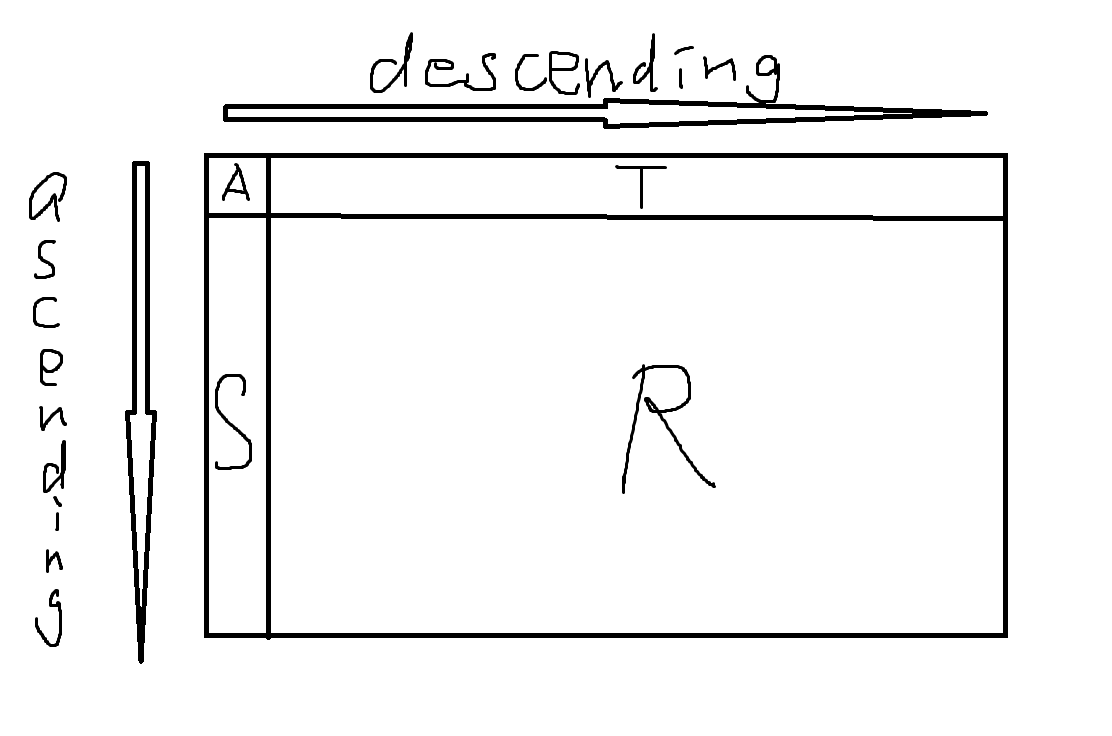
\includegraphics[width=0.4\textwidth]{matrix.png}
\end{figure}
~\\
\begin{enumerate}
    \item $A=X$, find it.
    \item $A<X$, $X$ is not in areas $A$ and $T$. Find $X$ in $[S,R]$.
    \item $A>X$, $X$ is not in areas $A$ and $S$. Find $X$ in $[T^T,R^T]^T$.
\end{enumerate}
\begin{minipage}[H]{0.8\textwidth}
\begin{algorithm}[H]
    \caption{Find-a-number-in-ordered-matrix}
    \label{matrix}
    \KwIn{A matrix $M$ with size $m\times n$; a target number $X$}
    \KwOut{The position of $X$, or "Not found"}
    \BlankLine
    \Function{Find(M, left, top, right, bottom, X)}{
        \BlankLine
        \If{$left > right$ \textbf{OR} $top > bottom$}{
            \Return{"Not Found"}
        }
        \If{$M(left,top)=X$}{
            \Return{$(left,top)$}
        }
        \If{$M(left,top)<X$}{
            \Return{Find$(M, left, top+1, right, bottom, X)$}
        }
        \If{$M(left,top)>X$}{
            \Return{Find$(M, left+1, top, right, bottom, X)$}
        }
    }
\end{algorithm}
\end{minipage}\\
Either $n$ or $m$ decreases by $1$ in one call. Therefore, $T(n,m)=\Theta(n+m)$.\\
Some other thoughts: 
\begin{itemize}
    \item Divide the matrix into $4$ parts equally. $T(4S)=3T(S)+1\Rightarrow T(S)=\Theta(3^{\log_4{S}})=\Theta((mn)^{\log_4{3}})$
    \item Traverse rows and binary search columns or traverse columns and binary search rows.\\ $T(n,m)=\Theta(\min\{n,m\}\log{\max\{n,m\}})$.
\end{itemize}
\end{solution}
~\\
\newpage
\item \textbf{Quicksort} is based on the Divide-and-Conquer method. Here is the two-step divide-and-conquer process for sorting a typical subarray $A[p \ldots r]$:
    \begin{enumerate}

    	\item
    	\textbf{Divide:} Partition the array $A[p \ldots r]$ into two subarrays $A[p \ldots q-1]$ and $A[q+1 \ldots r]$ such that each element of $A[p \ldots q-1]$ is less than or equal to $A[q],$ which is, in turn, less than or equal to each element of $A[q+1 \ldots r].$ Compute the index $q$ as part of this partitioning procedure.
    	
    	\item
    	\textbf{Conquer:} Sort $A[p \ldots q-1]$ and $A[q+1 \ldots r]$ respectively by recursive calls to Quicksort.
    	
    \end{enumerate}
    Write down the recurrence function $T(n)$ of QuickSort and compute its time complexity.

    {\color{purple}Hint: At this time $T(n)$ is split into two subarrays with different sizes (usually), and you need to describe its recurrence relation by the sum of two subfunctions plus additional operations.}

~\\
\begin{solution}
\begin{equation*}
T(n)=\left\{
    \begin{array}{ll}
        1&n=1\\
        n+\dfrac{1}{n}\sum_{i=1}^n{\left[T(i-1)+T(n-i)\right]}&n>1\\
    \end{array}
\right.
\end{equation*}\\
$T(n)=n+\dfrac{2}{n}\sum_{i=1}^{n-1}T(i)\Rightarrow nT(n)=n^2+2\sum_{i=1}^{n-1}T(i)$, therefore, $(n+1)T(n+1)=(n+1)^2+2\sum_{i=1}^nT(i)$\\
Therefore, $(n+1)T(n+1)=2n+1+(n+2)T(n)$, hence $\dfrac{T(n+1)-1}{n+2}=\dfrac{T(n)-1}{n+1}+\dfrac{2}{n+2}$\\
Therefore, $\dfrac{T(n+1)-1}{n+2}\sim 2\ln(n+1)\Rightarrow T(n)\sim 2n\ln n\Rightarrow T(n)=\Theta(n\log n)$.
\end{solution}
~\\


\textbf{Remark}: You need to upload your .pdf file and write the pseudocode.
\end{enumerate}

\end{document}
